\chapter{ Project Methods}
\label{chap:projectsteps}


\section{Introduce NoteSets as a new note data container}
\label{noteset_goal}
We will introduce so called \emph{NoteSets} as a new data container for referencing and persisting sets of note data. While these Note Sets will be exported to files, they do not constitute a file format \emph{strictu sensu}, but rather a new paradigm as how to think of collection of notes: Namely no longer as a group of notes that were recorded in the same transaction and thus reside in the same binary file (in earlier times this was the only way one could think of collections of notes), but rather as a collection of IDs that are linked by a common \emph{annotation}.

The note set data container will have the following advantages:
\begin{itemize}
\item Compactness: NoteSets will be minimalist in the sense that notes are referenced by ID only. There is no annotational information stored in the note set itself.
\item Independency of file locations: With the introduction of MFX the actual location of a file in the Data Lake becomes redundant. Therefore, the note set does not store any file paths.
\item Equivalence with respect to annotation: Unlike the Notelist format, NoteSets will no longer have an individual annotation per note. Rather, they have at most one annotation per NoteSet, which is to be persisted in the NoteSet's filename (cf. section \ref{ns_annotation_spec}). Thus, NoteSet are considered equivalent with respect to annotation
\end{itemize}
Meanwhile, the new data container must at least satisfy the following requirements:
\begin{itemize}
\item Convertability to and from the existing Notelist format. The Notelist format has been established as the standard way of storing data sets in Currency Adaptation. Even if one were to pursue the goal of replacing the Notelist format by the Noteset format, convertability would be needed at least for a period of transition.
 \item Operatability. Since they are so minimalist, Note Sets are more ideal than previous formats for quick comparison. We need a way to compare and find the difference between Note Sets reliably and efficiently. Furthermore we would like to do other set operations like union or intersection on NoteSets.
\end{itemize}

The NoteSet data container is introduced in a small Python library providing the abovementioned functionality. This library is deployed as a Python package and can be used in the Currency Adaptation Python toolchain, as well as in Jupyter notebooks. In a later step it remains to analyze the feasibility of introducing this data container in the .NET toolchain as well.

\section{Implement Processes for Automated NoteSet Generation}
In a first phase Jupyter Notebooks are used to generate the NoteSets. Different methods and their results, i.e. the resulting NoteSets, will be compared and presented to the Currency Adaptation Team. Once the NoteSet generation process has been refined on a technical level, it remains to decide how to implement it in the Currency Adaptation Software toolchain.\par
The NoteSet generation workflow in this development phase can be generalized as follows: 
\begin{enumerate}
\item Crawl MFX for a chosen directory in the Data Lake to obtain all File IDs. 
\item Query each note from MDS and determine it's annotation/label based on a chosen labeling method. 
\item Group all notes with the same annotation/label into NoteSets (within a NoteSet, all elements have the same label)
\end{enumerate}
It remains thus to choose a labeling method. The possible methods can be outlined as follows:
\begin{enumerate}
\item Query MDS to obtain the results calculated by the banknote reader for each note. In this case, we use the banknote reader (and the CDF which was loaded at the time of recording) as the labeller: For example, if the reader classified the note as e ``EUR 5 b Orientation 1`` at the time of recording, we will give it that label. This is the most straightforward way, since all that is done is query existing information from the MDS REST API. No new information is generated.
\item Use the MOVEmSimulator to simulate the banknote reader on the chosen set of notes and a chosen CDF. The results generated by the Simulator can then be used to group and label the Note Sets. This method is more complicated and time consuming than the first one, but it's also more generic, because it makes us independent from the CDF which was used in the original recording. For example, the original CDF used in the actual recording might classify a note as Category 3 (suspected counterfeit), but might now be outdated since the latest CDF for the same currency will classify the same note as Category 2 (proven counterfeit). On MDS, the information generated in the original recording is stored, therefore, this note will always be a Category 3 note if we use the first method. If we let the simulator process the chosen set of NIF files first, using the latest CDF, we will get the most up to date information, namely the results a physical reader would calculate using the most recently released CDF.
\item Computationally load all notes into MCM and use algorithm(s) from the MCM algorithmic framework to determine properties of each note based on which the notes can be labelled. In this case use MCM as the labeller. To access the MCM application from a Jupyter Notebook, a Python wrapper library for MCM has to be used.
\end{enumerate}
\par Figure \ref{fig:ns_mds} to \ref{fig:ns_mcm} visualizesthese different approaches.

\begin{figure}
\centering
\begin{subfigure}[b]{0.45\textwidth}
   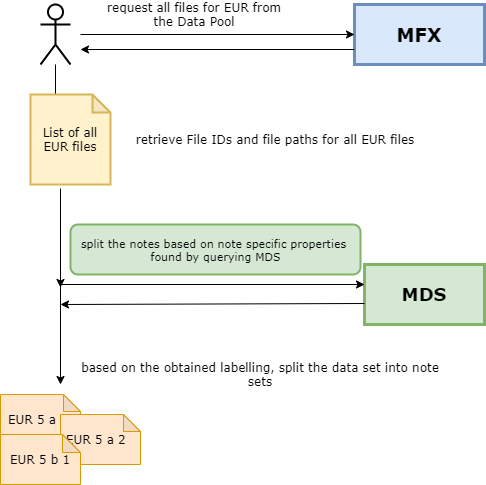
\includegraphics[width=1\linewidth]{images/label_mds_approach.png}
   \caption{NoteSet Generation with MDS labeling}
   \label{fig:ns_mds} 
\end{subfigure}

\begin{subfigure}[b]{0.45\textwidth}
   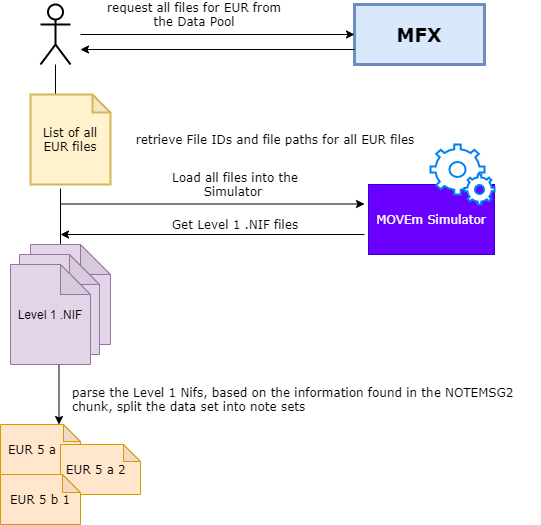
\includegraphics[width=1\linewidth]{images/label_simulator_approach.png}
   \caption{NoteSet Generation with MOVEm Simulator labeling}
   \label{fig:ns_sim}
\end{subfigure}

\begin{subfigure}[b]{0.45\textwidth}
   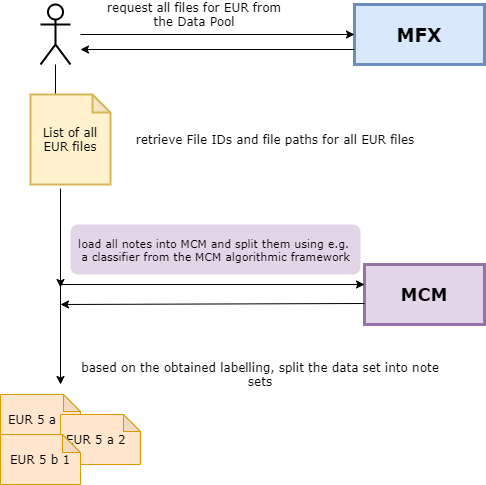
\includegraphics[width=1\linewidth]{images/label_mcm_approach.png}
   \caption{NoteSet Generation with MCM labeling}
   \label{fig:ns_mcm}
\end{subfigure}

\end{figure}

In the course of implementing the project the focus shifted almost entirely towards the method of labeling via MDS on the one hand and the MOVEm Simulator on the other. In a first stage I tried to use MCM as a labeller, but discarded this mainly because of performance reasons. MCM is already a very resource-intensive piece of software and accessing it via a Python wrapper from Jupyter had another negative impact on the performance. In addition, the python wrapper for MCM is quite limited as only a number of MCM functions are accessible and MCM is impossible to debug when accessed via Python. \par

\section{Introduce NoteSet loading in MCM}
Since MCM already uses MFX, it is able to load NIF files by File ID only, thus nothing stands in the way of loading Notes by ID, i.e. as a set of Note IDs. Therefore we want to extend MCM with a feature that allows loading and exporting of NoteSets. This should be done with as little cost as possible as introducing bigger changes and new models into MCM is always very complex and delicate. The idea is to allow passing NoteSets in the MCM View layer, but converting them into standard MCM Notelist objects before they are passed to deeper layers. 
